\chapter{Teoría de la dispersión}\label{ch:b3:scattering-theory}

Casi todo lo que sabemos de lo pequeño se ha aprendido lanzándole cosas y
mirando qué rebota. Rutherford descubrió el núcleo contando destellos de
partículas alfa sobre una pantalla de sulfuro de cinc; cincuenta años
después, el mismo experimento, realizado con electrones de mayor energía,
halló quarks dentro del protón; entre medias y desde entonces, toda \omterm{def:b3:scattering-theory:cross-section}{sección
eficaz} de la física nuclear, de partículas, atómica y de la materia
condensada se ha leído con la teoría de este capítulo. El lenguaje es la
\emph{\omterm{def:b3:scattering-theory:cross-section}{sección eficaz}} --- un área efectiva de blanco; el objeto cuántico es
la \emph{\omterm{thm:b3:scattering-theory:amplitude}{amplitud de dispersión}}, cuya \omterm{thm:b3:scattering-theory:born}{aproximación de Born} dice algo
inolvidable: un blanco difuso se sondea en el espacio de Fourier, ángulo a
ángulo. A baja energía toman el mando las \omterm{thm:b3:scattering-theory:partial}{ondas parciales}, que colapsan
cualquier potencial complicado en un solo número --- la \omterm{thm:b3:scattering-theory:partial}{longitud de
dispersión} --- que hoy sintoniza los gases cuánticos ultrafríos; y allí
donde un proyectil puede demorarse en un estado cuasiligado, la \omterm{def:b3:scattering-theory:cross-section}{sección
eficaz} se dispara en resonancias, la espectroscopia de lo que de otro modo
sería invisible.

\section{Secciones eficaces}

\begin{definition}[Sección eficaz]\label{def:b3:scattering-theory:cross-section}
\index{sección eficaz}\index{sección eficaz diferencial}
Envíese un haz uniforme de flujo $\Phi$ (partículas por unidad de área y de
segundo) sobre una partícula blanco. El ritmo de proyectiles dispersados
hacia el ángulo sólido $\dd\Omega$ alrededor de la dirección $(\theta,
\varphi)$ define la \emph{sección eficaz diferencial},
\[
\dd\dot N = \Phi\,\frac{\dd\sigma}{\dd\Omega}\,\dd\Omega ,
\]
y su integral $\sigma = \int(\dd\sigma/\dd\Omega)\,\dd\Omega$ es
la \emph{sección eficaz total}: el área que el blanco presenta
efectivamente. Para una lámina delgada con $n$ blancos por unidad de
volumen, un haz se atenúa como $\eu^{-n\sigma x}$: las secciones eficaces se
miden contando lo que emerge. Unidades: la física nuclear usa el
\emph{barn}, $\qty{1}{b} = \qty{e-28}{m^2}$ --- aproximadamente el tamaño
geométrico de un núcleo de uranio, ``grande como un granero'' para un
neutrón.
\end{definition}

\begin{omfigure}
\begin{tikzpicture}[font=\small, >=Stealth]
  % incident plane wave
  \foreach \x in {-4.6,-4.0,-3.4,-2.8}
    \draw[omDef] (\x,-1.15) -- (\x,1.15);
  \draw[->, omDef, very thick] (-4.5,1.5) -- (-2.9,1.5);
  \node[omDef, anchor=south] at (-3.7,1.55) {haz, flujo $\Phi$};
  % target
  \fill[omThm] (0,0) circle (3pt);
  \node[anchor=north, font=\footnotesize] at (0,-0.18) {blanco};
  % outgoing spherical
  \foreach \r in {0.7,1.3,1.9}
    \draw[omExo] (0,0) circle (\r);
  % detector
  \draw[->, thick] (0,0) -- (35:3.1);
  \draw[fill=omProp!25, draw=omProp, thick, rotate around={35:(35:3.4)}]
    ($(35:3.4)+(-0.12,-0.42)$) rectangle ($(35:3.4)+(0.12,0.42)$);
  \node[omProp, anchor=west, font=\footnotesize] at ($(35:3.4)+(0.25,0)$)
    {detector, $\dd\Omega$};
  \draw (1.15,0) arc (0:35:1.15);
  \node at (17:1.5) {$\theta$};
  \draw[->, thick] (0,0) -- (2.6,0);
\end{tikzpicture}

{\small El experimento de dispersión: una onda plana que entra, una onda
esférica que sale y un detector que cuenta en el ángulo $\theta$. El patrón
angular de las cuentas es la física del blanco.}
\end{omfigure}

\section{La amplitud y la aproximación de Born}

\begin{theorem}[Estados de dispersión y amplitud]\label{thm:b3:scattering-theory:amplitude}
\index{amplitud de dispersión}
Para una partícula de energía $E = \hbar^2k^2/2m$ que se encuentra con un
potencial localizado $V(\vect r)$, el estado estacionario de dispersión se
comporta a gran distancia como
\[
\psi(\vect r) \;\longrightarrow\;
\eu^{\iu kz} + f(\theta)\,\frac{\eu^{\iu kr}}{r} ,
\]
una onda plana incidente más una onda esférica saliente modulada por la
\emph{\omterm{thm:b3:scattering-theory:amplitude}{amplitud de dispersión}} $f(\theta)$ (una longitud), y
\[
\frac{\dd\sigma}{\dd\Omega} = |f(\theta)|^2 .
\]
\end{theorem}

\begin{proof}[Demostración parcial]
La caída en $1/r$ hace finito el flujo saliente a través de cualquier esfera
grande; al calcular las \omterm{prop:b3:schrodinger-three-dimensions:current}{corrientes de probabilidad}
(\cref{prop:b3:schrodinger-three-dimensions:current}) de los dos
términos, la corriente radial saliente por unidad de ángulo sólido es
$(\hbar k/m)|f|^2$ frente al flujo incidente $\hbar k/m$: el cociente
es la definición de $\dd\sigma/\dd\Omega$. Que existan soluciones de esta
forma asintótica se admite.
\end{proof}

\begin{theorem}[Aproximación de Born]\label{thm:b3:scattering-theory:born}
\index{aproximación de Born}\index{transferencia de momento}
Para un potencial débil (o un proyectil rápido), la \omterm{thm:b3:perturbation-theory:corrections}{teoría de
perturbaciones} de primer orden en $V$ da
\[
f(\theta) = -\frac{m}{2\pi\hbar^2}
\int V(\vect r)\,\eu^{\iu\vect q\cdot\vect r}\,\dd^3r ,
\qquad
\vect q = \vect k - \vect k' , \quad
q = 2k\sin\frac\theta2 :
\]
la amplitud es, salvo constantes, la \emph{transformada de Fourier del
potencial} evaluada en la \omterm{thm:b3:scattering-theory:born}{transferencia de momento} $\hbar\vect q$.
Los experimentos de dispersión son analizadores de Fourier de la materia:
los ángulos pequeños leen longitudes de onda largas (estructura gruesa) y
los grandes, el detalle fino --- la razón más profunda de que ``más energía''
signifique ``distancias más pequeñas''.
\end{theorem}

\begin{proof}[Demostración parcial]
Esto es la \omterm{thm:b3:perturbation-theory:golden}{regla de oro de Fermi}
(\cref{thm:b3:perturbation-theory:golden}) aplicada entre ondas planas
$\ket{\vect k} \to \ket{\vect k'}$: el elemento de matriz es
$\int V\eu^{\iu(\vect k - \vect k')\cdot\vect r}\dd^3r$, la
\omterm{prop:b3:schrodinger-three-dimensions:counting}{densidad de estados} finales suministra los factores cinemáticos y la
contabilidad (admitida) los ensambla en $f$. La elasticidad da
$|\vect k'| = |\vect k|$, de donde $q = 2k\sin(\theta/2)$ por el
triángulo isósceles de $\vect k, \vect k'$.
\end{proof}

\begin{example}[De Yukawa a Rutherford]\label{ex:b3:scattering-theory:rutherford}
\index{dispersión de Rutherford}
Para el potencial de Coulomb apantallado $V = \dfrac{Q_1Q_2}{4\pi
\varepsilon_0 r}\,\eu^{-r/a}$, la integral de Born es elemental
(\cref{exo:b3:scattering-theory:5}) y, cuando el radio de apantallamiento
$a \to \infty$,
\[
\frac{\dd\sigma}{\dd\Omega} =
\Big(\frac{Q_1Q_2}{16\pi\varepsilon_0 E}\Big)^2
\frac{1}{\sin^4(\theta/2)} :
\]
la \emph{\omterm{def:b3:scattering-theory:cross-section}{sección eficaz} de Rutherford}. Por una coincidencia exclusiva del
$1/r$, el cálculo clásico, la \omterm{thm:b3:scattering-theory:born}{aproximación de Born} y la respuesta cuántica
exacta coinciden todos --- razón por la cual Rutherford, calculando
clásicamente en 1911, obtuvo la fórmula correcta y, a partir de su
verificación destello a destello, el núcleo
(\cref{pb:b3:scattering-theory:1}).
\end{example}

\section{Ondas parciales y longitud de dispersión}

\begin{theorem}[Desfases]\label{thm:b3:scattering-theory:partial}
\index{ondas parciales}\index{desfase}\index{longitud de dispersión}
Para un potencial central, descompóngase el estado de dispersión en
momentos angulares: cada onda parcial $l$ abandona la región del potencial
con su oscilación radial \emph{desplazada} en una fase $\delta_l(k)$
--- la atracción la adelanta y la repulsión la retrasa --- y la amplitud
observable se recompone como
\[
f(\theta) = \frac1k\sum_{l=0}^\infty(2l+1)\,\eu^{\iu\delta_l}
\sin\delta_l\,P_l(\cos\theta) , \qquad
\sigma = \frac{4\pi}{k^2}\sum_l(2l+1)\sin^2\delta_l .
\]
A baja energía, la intuición clásica ($l \sim kb$ para un parámetro de
impacto $b$) dice que solo penetra $l = 0$: la dispersión se vuelve
isótropa y un solo número manda,
\[
f \to -a , \qquad \sigma \to 4\pi a^2 ,
\]
donde $a = -\lim_{k\to0}\delta_0/k$ es la \emph{\omterm{thm:b3:scattering-theory:partial}{longitud de
dispersión}}. Sea cual sea su complejidad interna, a baja energía un blanco
\emph{es} su \omterm{thm:b3:scattering-theory:partial}{longitud de dispersión} --- la gran simplificación sobre la que
funciona la física de átomos fríos.
\end{theorem}
\admitted

\begin{omfigure}
\begin{tikzpicture}
  \begin{axis}[omaxis, axis x line=bottom, axis y line=left,
    width=11.6cm, height=5.2cm, xmin=0, xmax=12.3, ymin=-1.5, ymax=1.5,
    xlabel={$r$}, ylabel={$u_0(r)$},
    xlabel style={at={(axis description cs:0.5,-0.1)}, anchor=north},
    xtick=\empty, ytick=\empty, clip=false]
    \addplot[gray, dashed, domain=0:12.3, samples=200] {sin(deg(x))};
    \addplot[omDef, very thick, domain=1.9:12.3, samples=200] {sin(deg(x+0.9))};
    \draw[omExo, thick] (axis cs:0,-1.5) -- (axis cs:0,1.5);
    \fill[omExo!14] (axis cs:0,-1.5) rectangle (axis cs:1.9,1.5);
    \node[font=\scriptsize, anchor=south] at (axis cs:0.95,1.12) {región del};
    \node[font=\scriptsize, anchor=south] at (axis cs:0.95,0.78) {potencial};
    \draw[<->, omThm, thick] (axis cs:8.51,-1.28) -- (axis cs:9.42,-1.28);
    \node[omThm, font=\scriptsize, anchor=north] at (axis cs:8.95,-1.32)
      {desplazamiento $\delta_0/k$};
    \node[gray, font=\scriptsize, anchor=west] at (axis cs:10.7,1.28) {libre};
    \node[omDef, font=\scriptsize, anchor=west] at (axis cs:10.55,0.92) {dispersada};
  \end{axis}
\end{tikzpicture}

{\small Una onda parcial abandona la región de interacción con su
oscilación desplazada: el desfase $\delta_0$. Todo lo que un detector puede
saber de un potencial central a una energía dada es la lista de esos
desfases.}
\end{omfigure}

\begin{example}[El neutrón se encuentra con el protón]\label{ex:b3:scattering-theory:np}
Los neutrones lentos se dispersan en protones con $\sigma \approx
\qty{20.4}{b}$ --- un área cuarenta veces mayor que el tamaño geométrico del
deuterón. La explicación: la colisión de baja energía es onda $s$ pura
con dos canales de espín, cuyas \omterm{thm:b3:scattering-theory:partial}{longitudes de dispersión} medidas,
$a_{\text{t}} = \qty{5.4}{fm}$ (triplete) y $a_{\text{s}} =
\qty{-23.7}{fm}$ (singlete), son ambas mucho mayores que el alcance de
\qty{2}{fm} de la fuerza. Un $|a|$ grande significa un estado \emph{casi}
a energía nula: el deuterón apenas ligado del triplete
(\cref{ex:b3:schrodinger-three-dimensions:deuteron}) y, en el
singlete, un compañero ``virtual'' que no llega a ligarse --- su
fracaso escrito en $a_{\text{s}} < 0$. Un enigma de veinte barns,
resuelto por dos estados ligados a punto de existir
(\cref{exo:b3:scattering-theory:7}).
\end{example}

\section{Resonancias}

\begin{proposition}[Resonancias de Breit--Wigner]\label{prop:b3:scattering-theory:resonance}
\index{resonancia!de dispersión}\index{fórmula de Breit--Wigner}
Si el proyectil puede quedar capturado temporalmente en un estado
cuasiligado de energía $E_{\text{R}}$ y vida media $\tau = \hbar/\Gamma$,
el desfase correspondiente barre $\pi/2$ y la \omterm{def:b3:scattering-theory:cross-section}{sección eficaz} parcial se
dispara:
\[
\sigma_l(E) \approx \frac{4\pi}{k^2}\,(2l+1)\,
\frac{\Gamma^2/4}{(E - E_{\text{R}})^2 + \Gamma^2/4} ,
\]
un pico lorentziano de anchura $\Gamma$ en el techo que la onda puede
alcanzar (el ``límite de unitariedad'' $4\pi(2l+1)/k^2$). Leída al revés,
una resonancia en una \omterm{def:b3:scattering-theory:cross-section}{sección eficaz} \emph{es} el descubrimiento de un
estado: su posición es un nivel de energía y su anchura, una vida media. La
mayor parte del zoo de partículas del \cref{ch:b3:particle-physics} se
descubrió como jorobas de esta clase.
\end{proposition}
\admitted

\begin{omfigure}
\begin{tikzpicture}
  \begin{axis}[omaxis, axis x line=bottom, axis y line=left,
    width=7.0cm, height=5.0cm, xmin=0, xmax=10, ymin=0, ymax=1.2,
    xlabel={$E$}, ylabel={$\sigma$ (a escala)},
    xlabel style={at={(axis description cs:0.5,-0.11)}, anchor=north},
    xtick={4}, xticklabels={$E_{\text{R}}$}, ytick=\empty, clip=false]
    \addplot[omDef, very thick, domain=0:10, samples=200]
      {0.06 + 0.25/((x-4)^2+0.27)};
    \draw[<->, omThm] (axis cs:3.48,0.53) -- (axis cs:4.52,0.53);
    \node[omThm, font=\scriptsize, anchor=south] at (axis cs:4.0,0.56) {$\Gamma$};
  \end{axis}
  \begin{axis}[omaxis, axis x line=bottom, axis y line=left,
    width=7.0cm, height=5.0cm, xmin=0, xmax=10, ymin=0, ymax=1.2,
    xshift=7.6cm,
    xlabel={$E$ (eV)}, ylabel={$\sigma$ (a escala)},
    xlabel style={at={(axis description cs:0.5,-0.11)}, anchor=north},
    xtick={1}, ytick=\empty, clip=false]
    \addplot[omExo, very thick, domain=0.05:10, samples=250]
      {0.75*((x-1)*(x-1)+0.06)/(x*x*0.35+0.5)+0.02};
    \node[omExo, font=\scriptsize, anchor=west] at (axis cs:1.15,0.14)
      {ventana de transparencia};
  \end{axis}
\end{tikzpicture}

{\small Dos caras del desfase. Izquierda: un estado cuasiligado
hace barrer a $\delta$ por $\pi/2$ --- un pico de Breit--Wigner cuya
anchura es una vida media. Derecha: el efecto Ramsauer--Townsend --- en el
argón, $\delta_0$ pasa por $\pi$ cerca de \qty{1}{eV} y el
átomo se vuelve casi transparente a los electrones: interferencia
destructiva como antirresonancia.}
\end{omfigure}

\begin{method}[Leer un problema de dispersión]\label{met:b3:scattering-theory:method}
(1) Primero la cinemática: $k$ y el rango accesible de $q$, $0 \le q
\le 2k$ --- ¿qué escalas de estructura son visibles? (2) Rápido y débil:
Born --- transfórmese Fourier el potencial y compruébese la pequeñez. (3)
Lento: \omterm{thm:b3:scattering-theory:partial}{ondas parciales}, normalmente solo la $s$; piénsese en la \omterm{thm:b3:scattering-theory:partial}{longitud de
dispersión} y espérese $\sigma = 4\pi a^2$ (para \omterm{def:b3:identical-particles:exchange}{partículas idénticas}
bosónicas: $8\pi a^2$). (4) Picos en $\sigma(E)$: ajústese Breit--Wigner y
comuníquese un nivel y una vida media; valles: una fase que pasa por $\pi$.
(5) Blancos extensos: multiplíquese la amplitud puntual por el factor de
forma --- la transformada de Fourier de la densidad
(\cref{exo:b3:scattering-theory:12}).
\end{method}

\begin{omfigure}
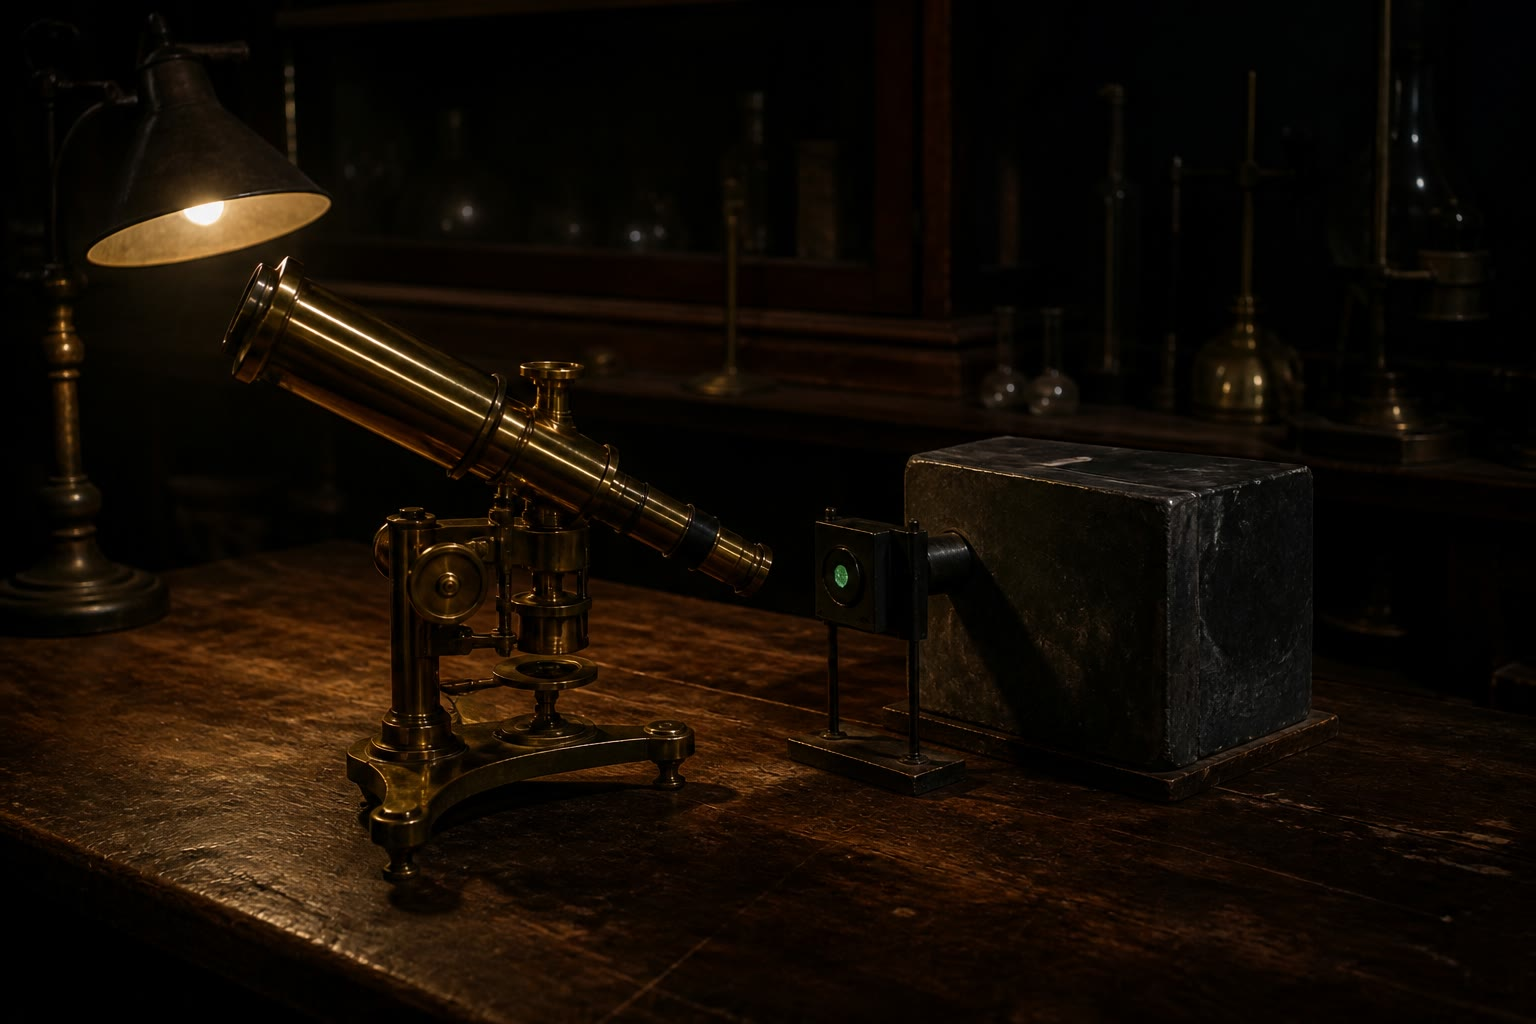
\includegraphics[width=0.58\linewidth]{images/book5/ai/b5-15-scintillation-lab.jpg}

{\small El primer laboratorio de dispersión: un microscopio de latón apuntado a una pantalla de sulfuro de cinc, contando un tenue destello verde por cada partícula $\alpha$ que llega. A partir de esas cuentas, ángulo a ángulo, Rutherford pesó el corazón del átomo.}
\end{omfigure}

\section{Ejercicios}

\begin{exercise}[$\star$]\label{exo:b3:scattering-theory:1}
Un haz de protones de \qty{1}{\micro A} ($\num{6.2e12}$ protones/s) y
sección \qty{1}{cm^2} atraviesa una lámina de oro de \qty{1}{\micro m} ($n =
\qty{5.9e28}{m^{-3}}$). (a) La densidad superficial de blancos. (b) Con
$\sigma = \qty{10}{b}$ por núcleo, ¿qué fracción del haz se
dispersa? (c) El ritmo hacia un detector de ángulo sólido
\qty{e-3}{sr} si la dispersión fuera isótropa. (d) ¿Por qué es la
``\omterm{def:b3:scattering-theory:cross-section}{sección eficaz}'' una propiedad bien definida de la \emph{terna}
(proyectil, blanco, energía) y no del blanco por sí solo?
\end{exercise}

\begin{exercise}[$\star$]\label{exo:b3:scattering-theory:2}
Esferas duras clásicas de radios $R_1, R_2$: (a) muéstrese que $\sigma =
\pi(R_1 + R_2)^2$. (b) Para las moléculas del aire ($R \approx
\qty{0.15}{nm}$, $n = \qty{2.5e25}{m^{-3}}$), el recorrido libre medio
$1/n\sigma$: evalúese y compárese con el valor de la teoría cinética
del volumen del Año 1. (c) ¿Por qué no muestra una esfera dura clásica
estructura angular ($\dd\sigma/\dd\Omega$ constante --- acéptese o
dedúzcase)? (d) ¿Qué rasgo de la dispersión \emph{cuántica} por esfera dura
(\cref{exo:b3:scattering-theory:6}) no tiene contrapartida clásica?
\end{exercise}

\begin{exercise}[$\star$]\label{exo:b3:scattering-theory:3}
\omterm{thm:b3:scattering-theory:born}{Transferencia de momento}. (a) Dibújese el triángulo de $\vect k$ y $\vect k'$
y dedúzcase $q = 2k\sin(\theta/2)$. (b) Para alfas de \qty{5.5}{MeV}
($k = \qty{1.0e15}{m^{-1}}$): el rango de $q$ para $\theta \in
[0, \pi]$ y la estructura más pequeña resoluble $\sim 1/q_{\max}$.
(c) Para electrones de \qty{500}{MeV} ($k \approx E/\hbar c$): lo mismo.
(d) Extráigase la moraleja que conecta la energía del haz con la potencia de
resolución.
\end{exercise}

\begin{exercise}[$\star$]\label{exo:b3:scattering-theory:4}
A partir del \cref{thm:b3:scattering-theory:amplitude}: (a) compruébese que
$|f|^2$ tiene dimensiones de área por unidad de ángulo sólido; (b) muéstrese
que el flujo dispersado a través de una esfera vale $\Phi\sigma$; (c) ¿por
qué debe ser $f$ complejo en general (qué ley de conservación custodia su
fase)? (d) Enúnciense el teorema óptico $\sigma_{\text{tot}} =
(4\pi/k)\operatorname{Im}f(0)$ y su significado (la onda hacia delante debe
quedar mermada exactamente en lo que se dispersa fuera).
\end{exercise}

\begin{exercise}[$\star\star$]\label{exo:b3:scattering-theory:5}
Born para Yukawa. Con $V(r) = \dfrac{g\,\eu^{-\mu r}}{r}$: (a)
realícese la integral de Born (primero la parte angular y luego $\int_0^
\infty\sin(qr)\eu^{-\mu r}\dd r$) para obtener $f = -\dfrac{2mg}
{\hbar^2(q^2 + \mu^2)}$. (b) Hágase $\mu \to 0$ con $g =
Q_1Q_2/4\pi\varepsilon_0$ y recupérese Rutherford. (c) ¿Por qué diverge la
\omterm{def:b3:scattering-theory:cross-section}{sección eficaz} \emph{total} de Rutherford, y qué ingrediente físico (el
apantallamiento por los electrones atómicos) restituye una respuesta
finita? (d) En física de partículas, la forma de Yukawa con $\mu =
m_\pi c/\hbar$ modeliza la fuerza nuclear: calcúlese su alcance
$1/\mu$ para $m_\pi c^2 = \qty{140}{MeV}$.
\end{exercise}

\begin{exercise}[$\star\star$]\label{exo:b3:scattering-theory:6}
La esfera dura cuántica (de radio $a$), onda $s$: fuera, $u_0 =
\sin(kr + \delta_0)$ con $u_0(a) = 0$. (a) Muéstrese que $\delta_0 = -ka$.
(b) Muéstrese que $\sigma \to 4\pi a^2$ cuando $k \to 0$: \emph{cuatro}
veces la sombra geométrica. (c) Dese la explicación ondulatoria del factor
(la difracción no deja sombra nítida con longitudes de onda largas). (d) A
alta energía la respuesta tiende a $2\pi a^2$ --- todavía el doble de la
geométrica (difracción de sombra): ¿por qué nunca simplemente $\pi a^2$?
\end{exercise}

\begin{exercise}[$\star\star$]\label{exo:b3:scattering-theory:7}
Los veinte barns del hidrógeno. Los neutrones lentos no polarizados sobre
protones muestrean el canal triplete con peso $3/4$ y el
singlete con $1/4$: $\sigma = \pi(3a_{\text{t}}^2 +
a_{\text{s}}^2)$. (a) Evalúese con $a_{\text{t}} = \qty{5.4}{fm}$ y
$a_{\text{s}} = \qty{-23.7}{fm}$, y compárese con los \qty{20.4}{b}
medidos. (b) ¿Qué canal domina, pese a su menor peso
estadístico? (c) Relaciónense el tamaño y el signo de $a_{\text{t}}$ con la
energía de enlace casi nula del deuterón; ¿qué dice $a_{\text{s}} < 0$
sobre el sistema singlete? (d) ¿Por qué es el agua un moderador tan eficaz
de los neutrones de reactor, y por qué le importa esta \omterm{def:b3:scattering-theory:cross-section}{sección eficaz}?
\end{exercise}

\begin{exercise}[$\star\star$]\label{exo:b3:scattering-theory:8}
Ramsauer--Townsend. Modelícese el átomo de argón, para un electrón
entrante, como un pozo cuadrado atractivo de alcance $R =
\qty{0.2}{nm}$. (a) Dentro, el número de ondas es $K =
\sqrt{2m(E + V_0)}/\hbar$: el empalme puede hacer que la onda exterior
emerja con $\delta_0 = \pi$ exactamente --- ¿cuál es entonces la \omterm{def:b3:scattering-theory:cross-section}{sección
eficaz} de onda $s$? (b) ¿Por qué se vuelve el átomo casi invisible a esa
energía, aunque el pozo sea intenso? (c) Estímese el $V_0$
que sitúa la transparencia cerca de $E = \qty{1}{eV}$ (hágase que el pozo
albergue media longitud de onda: $KR \approx \pi$). (d) ¿Por qué \emph{no}
muestran el efecto el helio y el neón a energías comparables (sus pozos son
demasiado someros para que $\delta_0$ alcance $\pi$), y qué demuestra sobre
las ondas de materia la mera existencia del efecto?
\end{exercise}

\begin{exercise}[$\star\star$]\label{exo:b3:scattering-theory:9}
Para una amplitud de onda $s$ pura $f = \eu^{\iu\delta_0}\sin\delta_0/
k$: (a) calcúlese $\sigma$; (b) calcúlese $(4\pi/k)\operatorname{Im}
f(0)$ y verifíquese el teorema óptico; (c) muéstrese que la \omterm{def:b3:scattering-theory:cross-section}{sección eficaz}
máxima de onda $s$ es $4\pi/k^2$ (el límite de unitariedad) y
evalúese para neutrones térmicos ($k = \qty{3.1e10}{m^{-1}}$) en
barns; (d) ¿por qué no puede una resonancia empujar $\sigma_0$ más allá de
ese techo, por intensa que sea la interacción?
\end{exercise}

\begin{exercise}[$\star\star\star$]\label{exo:b3:scattering-theory:10}
Una resonancia neutrónica. El uranio-238 presenta una resonancia célebre
para neutrones en $E_{\text{R}} = \qty{6.67}{eV}$ con anchura total
$\Gamma = \qty{27}{meV}$. (a) Calcúlese la vida media de la resonancia.
(b) Calcúlese $4\pi/k^2$ a esa energía, en barns, y compárese con
el pico medido de $\sim\qty{2e4}{b}$ (la diferencia es el factor de
ramificación entre los canales elástico y de captura ---
coméntese). (c) La anchura en unidades de temperatura: ¿por qué importa
para la estabilidad del reactor el ensanchamiento Doppler de esta resonancia
con la temperatura del combustible (qué signo de realimentación)? (d) En dos
frases: cómo hacen tales resonancias del $^{238}$U un absorbedor de
neutrones en el rango epitérmico, y por qué es eso central en el diseño de
reactores.
\end{exercise}

\begin{exercise}[$\star\star\star$]\label{exo:b3:scattering-theory:11}
Los átomos fríos viven de un solo número. (a) Para bosones idénticos, la
\omterm{def:b3:scattering-theory:cross-section}{sección eficaz} de baja energía es $8\pi a^2$ (interferencia constructiva de
intercambio --- acéptese): evalúese para el rubidio con $a =
100\,a_0$. (b) A $T = \qty{100}{nK}$, compruébese que $ka \ll 1$
(calcúlese $k$ a partir de $k_{\text{B}}T = \hbar^2k^2/2m$, con $m =
\qty{1.4e-25}{kg}$): el gas olvida de verdad todo salvo $a$.
(c) Cerca de una resonancia ``de Feshbach'', un campo magnético arrastra un
nivel molecular a través de la energía cero y $a$ diverge y cambia de
signo, exactamente como en el \cref{ex:b3:scattering-theory:np}: ¿en qué se
convierten a voluntad las interacciones del gas? (d) ¿Por qué es esa
sintonizabilidad --- la intensidad de la interacción en un dial --- un
instrumento de ensueño para un físico (nómbrese un uso: fabricar moléculas,
simular materia fuertemente acoplada o colapsar condensados)?
\end{exercise}

\begin{exercise}[$\star\star\star$]\label{exo:b3:scattering-theory:12}
Factores de forma: pesar nubes de carga. Para una densidad de carga
extensa $\rho(\vect r)$, la amplitud de Born multiplica la respuesta puntual
por $F(q) = \int\rho(\vect r)\eu^{\iu\vect q\cdot\vect r}
\dd^3r/Q$. (a) Muéstrese que $F(0) = 1$. (b) Desarróllese para $q$ pequeño: $F
\approx 1 - q^2\langle r^2\rangle/6$: medir la caída a $q$ pequeño pesa
$\langle r^2\rangle$. (c) La dispersión electrón--protón ajusta
$\sqrt{\langle r^2\rangle} \approx \qty{0.84}{fm}$: ¿qué medida
independiente del \cref{pb:b3:hydrogen-atom:1} (el hidrógeno muónico) la
contrasta, y por qué se tomó tan en serio su desacuerdo histórico (el
``enigma del radio del protón'')? (d) Para $q \gg 1/r_{\text{p}}$, el
factor de forma elástico se desploma, pero la dispersión dura persiste sobre
\emph{constituyentes puntuales}: enúnciese en una frase qué halló dentro del
protón la versión profundamente inelástica del experimento de Rutherford, en
1968.
\end{exercise}

\section{Problema: los contadores de destellos que hallaron el núcleo}

\begin{problem}[{Problema de fin de semana --- la dispersión de Rutherford,
de la geometría a los quarks}]\label{pb:b3:scattering-theory:1}
En 1909, Geiger y Marsden pasaban las horas a oscuras contando destellos de
centelleo: partículas alfa disparadas a través de una lámina de oro, unas
pocas de las cuales rebotaban casi hacia atrás --- ``como si un proyectil
hubiera rebotado en un papel de seda''. El análisis que Rutherford hizo de
esas cuentas en 1911 creó el átomo nuclear. Este problema lo reconstruye.
Datos: energía del alfa $E =
\qty{5.5}{MeV}$ y carga $z = 2$; oro con $Z = 79$, espesor de lámina $t
= \qty{0.4}{\micro m}$ y una densidad atómica $n = \qty{5.9e28}{m^{-3}}$; $k_C =
1/4\pi\varepsilon_0 = \qty{8.99e9}{N.m^2/C^2}$.

\medskip\noindent\textbf{Parte I --- Un alfa, un núcleo.}
\begin{enumerate}
  \item En la imagen del pudin de pasas (con la carga repartida por el
        átomo, \qty{e-10}{m}), estímese la desviación máxima que un solo
        átomo podría imprimir a un alfa de \qty{5.5}{MeV} (campo de una
        esfera difuminada: $\theta \sim$ fuerza $\times$ tiempo / momento
        $\sim 2Zze^2k_C/(E\cdot\qty{e-10}{m})$ en radianes). ¿Podría
        cualquier acumulación de tales impulsos enviar alfas hacia atrás?
  \item Sea ahora la carga puntual. Escríbase la distancia de máxima
        aproximación $d_0$ para una colisión frontal (toda la energía
        cinética convertida en energía de Coulomb) y evalúese.
  \item ¿Qué implica, por tanto, \emph{de inmediato} un ritmo medible de
        dispersión casi hacia atrás sobre lo concentrada que está la
        carga positiva del átomo?
  \item Para un parámetro de impacto $b$ genérico, la órbita clásica da
        $\tan(\theta/2) = d_0/2b$ (admitido --- la hipérbola del capítulo
        de gravitación del volumen del Año 1, con repulsión): compruébense
        sus límites en $b \to 0$ y en $b \to
        \infty$.
  \item Calcúlense el parámetro de impacto que dispersa un alfa más de
        $90^\circ$, y la fracción de alfas que atraviesan la lámina y
        se acercan tanto a algún núcleo ($n t\,\pi
        b^2$).
  \item Geiger y Marsden hallaron cerca de 1 de cada 8000 alfas desviado
        más de $90^\circ$: compárese.
\end{enumerate}

\medskip\noindent\textbf{Parte II --- La \omterm{def:b3:scattering-theory:cross-section}{sección eficaz}.}
\begin{enumerate}[resume]
  \item Los alfas con parámetro de impacto en $[b, b + \dd b]$ se
        dispersan hacia $[\theta, \theta + \dd\theta]$: de $\dd\sigma =
        2\pi b\,|\dd b|$ y de la relación de la órbita, dedúzcase
        \[
        \frac{\dd\sigma}{\dd\Omega} =
        \Big(\frac{d_0}{4}\Big)^2\frac{1}{\sin^4(\theta/2)} .
        \]
  \item Verifíquese que coincide con la respuesta cuántica y de Born del
        \cref{ex:b3:scattering-theory:rutherford} (reescriba $d_0$
        en función de $E$).
  \item Evalúese $\dd\sigma/\dd\Omega$ en $\theta = 30^\circ$,
        $60^\circ$ y $120^\circ$ (en barns por estereorradián).
  \item Las cuentas de Geiger y Marsden de 1913, con geometría fija,
        escalan como $1{:}\,\sin^{-4}(\theta/2)$: calcúlese la razón de
        cuentas prevista entre $30^\circ$ y $120^\circ$ y
        obsérvese que sus datos siguieron esas razones a lo largo de cinco
        órdenes de magnitud de ritmo.
  \item ¿Por qué permite el $Z^2$ de esa misma fórmula que el experimento
        \emph{pese} la carga nuclear, y cómo ayudaron tales ajustes a
        fijar el $Z$ (el oro: 79) como número atómico?
  \item El $1/E^2$: ¿qué le ocurre a todo el patrón angular cuando se
        duplica la energía del alfa?
\end{enumerate}

\medskip\noindent\textbf{Parte III --- El tamaño del núcleo.}
\begin{enumerate}[resume]
  \item Aproximación máxima en el ángulo $\theta$: $d(\theta) =
        \tfrac{d_0}2[1 + 1/\sin(\theta/2)]$ (admitido). Evalúese
        para $\theta = 180^\circ$ y \qty{60}{\degree}.
  \item Mientras $d(\theta)$ supere el radio nuclear, la fórmula de carga
        puntual se cumple: ¿qué cota superior al tamaño del núcleo de oro
        establecieron los puntos a $180^\circ$ verificados por
        Rutherford?
  \item Con proyectiles de más energía, las cuentas a gran ángulo
        \emph{caen por debajo} de Rutherford: ¿qué señala esa desviación
        (qué fuerza nueva y a qué distancia)?
  \item La dispersión moderna de electrones da radios nucleares $R
        \approx r_0A^{1/3}$ con $r_0 = \qty{1.2}{fm}$: evalúese
        para el oro ($A = 197$) y compárese con su cota.
  \item El $A^{1/3}$: ¿qué dice sobre la densidad de la materia nuclear
        (¿constante?, ¿creciente?) --- un hecho sobre el que construirá el
        \cref{ch:b3:nuclear-physics}?
  \item ¿Por qué murió el modelo del pudin de pasas (ciego a la carga) a
        causa de \emph{este} experimento y no de la espectroscopia?
\end{enumerate}

\medskip\noindent\textbf{Parte IV --- Los nietos de Rutherford.}
\begin{enumerate}[resume]
  \item Enumérese la tabla exacta de traducción entre 1911 y 1968:
        alfa $\to$ haz de electrones, átomo de oro $\to$ protón,
        núcleo $\to$ quarks --- ¿qué hizo el papel de los ``sucesos
        inesperados a gran ángulo'' en el SLAC?
  \item ¿Por qué son los \emph{electrones} la sonda más limpia (qué
        complicación de la dispersión alfa--núcleo no tienen)?
  \item En lenguaje de Born: la dispersión elástica a $q$ alto mide el
        desplome del factor de forma (una nube blanda), mientras que los
        ritmos profundamente inelásticos siguieron siendo grandes y casi
        puntuales: enúnciese la conclusión que se extrajo.
  \item El arco de un siglo en tres filas: dense (energía de la sonda,
        distancia resuelta) para los alfas de 1911 ($\sim\qty{e-14}{m}$),
        el SLAC de 1968 (\qty{20}{GeV}, $\sim\qty{e-16}{m}$) y el
        LHC (escala del TeV, $\sim\qty{e-19}{m}$) --- usando
        la regla ``resolución $\sim \hbar c/(qc)$''.
  \item Los neutrones, sin carga, se dispersan solo en los núcleos (y en
        los momentos magnéticos): nómbrense dos cosas que la dispersión de
        neutrones cartografía, por tanto, en los materiales y que los
        rayos X ven mal (los átomos ligeros, como el hidrógeno; el orden
        magnético).
  \item Las secciones eficaces de descubrimiento en el LHC se miden en
        \emph{femtobarns} ($\qty{e-43}{m^2}$): del barn al
        femtobarn hay quince órdenes de magnitud --- ¿qué dice eso sobre
        lo raras que son las colisiones interesantes, y por qué es la
        luminosidad (el flujo entregado) tan preciosa como la energía?
  \item Resúmase el resultado con nombre propio: una ley en
        $\sin^{-4}(\theta/2)$, verificada destello a destello, metió el
        $99.98\%$ de la masa del átomo en un volumen $10^{-14}$ veces su
        tamaño --- y el mismo experimento, repetido cada vez con más
        fuerza, no ha dejado de encontrar la capa siguiente.
\end{enumerate}
\end{problem}
